\section{Intrusion Prevention Systems setup}
It is explicitly required in the assignment to actually set up \textbf{Intrusion Prevention Systems}, so that they can not only detect intruders raising an alarm, but also perform actions in order to prevent the intrusion, like dropping suspicious packets. We are going to set up two different systems: in the two firewalls, we exploit the \textbf{suricata} service provided by the \textbf{OPNSense} administration panel to build a \textbf{Network Intrusion Prevention System}, while in the two hosts of the \textbf{DMZ subnetwork}, we download and configure the \textbf{fail2ban} tool to build a \textbf{Host Intrusion Prevention System}.\\
The differences and analogies between the two systems will be clear in the next two subparagraphs, as well as their configurations and functionalities.\\

\subsection{suricata}
The \textbf{suricata} service can be enabled in the \textbf{OPNSense} administration panel by navigating to \textit{System -$>$ Services -$>$ Intrusion Detection -$>$ Administration}. For both routers, we enable the service and we also check the box \textbf{IPS} to make it possible for the service to actually \textit{drop packets} matching a rule, so that it will not only raise an alarm, but also perform some concrete action in preventing the intrusion.\\
For both of them we also enable the \textbf{promiscuous mode} so that the systems will also monitor and check the rules for packets that are not strictly directed to one of their interfaces - so, obviously, forward packets will also be checked - and the \textbf{logging} service.\\
In the \textbf{Main Router}, we enable the service for \textit{all the interfaces, but the WAN interface}. This latter interface indeed is probably the one seeing the most of the traffic, being connected to the Internet, so we decide to run the system only at the interfaces directly connected to our services, so that when packets get there they have already been checked against the WAN interface's firewall rules and the interface itself won't be a bottleneck to the whole network just by checking every packet to every single rule of the \textbf{NIPS}.\\
In the \textbf{Internal Router}, the very same logic is applied and thus the service is only enabled on the \textbf{CLIENTS} and \textbf{SERVERS} interfaces.\\
Both systems in both firewalls are configured to update their rules daily according to a given schedule. Both of them will drop packets matching against one of the rules that have been selected.\\
The rulesets that are enabled follow below - and they are almost the same for both to apply defense-in-depth for the most internal firewall:\\

\begin{itemize}
\item all the rulesets from \textbf{Abuse.ch}, except \textit{Feodo Tracker}. These rules should detect compromised websites distributing malware, compromised and bad SSL certificates and such;
\item \textbf{ETOpen Attack-Response} catching common results of successful attacks;
\item \textbf{ETOpen botcc} for detecting Botnets and C2 hosts;
\item \textbf{ETOpen DOS} rules for DoS attacks;
\item \textbf{ETOpen DROP} rules for spam activities;
\item \textbf{ETOpen Exploit} and \textbf{ETOpen Malware} for detecting general exploits and malwares;
\item \textbf{ETOpen Inappropriate} rules for detecting accesses to inappropriate websites;
\item \textbf{ETOpen Policy} rules containing checks for things that are usually not enabled by a company policy - that seemed our case;
\item \textbf{ETOpen Scan} rules to prevent network scans, probes and in general reconnaissance activities;
\item \textbf{ETOpen Web rules} - \textit{client} in the Internal firewall, \textit{client and server} at the Main firewall, for web application security and prevention of common attacks - such as SQL injection, XSS;
\item finally, we also included some rules from the \textbf{OPNSense Suricata Application Detection}, namely for \textbf{file$-$transfer} and \textbf{mailing} applications - once again, it seemed our case to include these rulesets given the network belongs to a company, and clients are likely to be exploiting such applications.
\end{itemize}

The two routers do not seem to be overloaded by the rulesets that were applied, even if they are quite a lot and some might also be unnecessary - \textbf{botcc} and maybe the \textbf{Inappropriate} rules, the latter especially given the proxy and DNS service we set up previously.\\

\subsection{fail2ban}
The \textbf{fail2ban} tool can be downloaded on both the two machines running in the \textbf{DMZ}, namely the \textbf{proxy machine} and the \textbf{web machine}. We have three different services running on these machines, whose access we want to protect with this tool:

\begin{itemize}
\item \textbf{SSH} service running on both;
\item \textbf{apache2} service running on the \textbf{web machine};
\item \textbf{squid} service running on the \textbf{proxy machine};
\end{itemize}

so we copy the content of file \textit{$/$etc$/$fail2ban$/$jail.conf} in a new file, \textit{jail.local} under the same directory, which will be now used by \textbf{fail2ban} as configuration file for its jail. We leave unmodified the preconfigured values for parameters such as \textit{bantime} and \textit{maxretry} - 3600 and 5 - and we do not specify in neither of the two configurations for the two machines IP addresses that we want to ignore in the field \textit{ignoreip}, apart from the local loop, so that especially in the case of the \textbf{squid} service, we will monitor also accesses coming from the Clients subnetwork, so to prevent possible physical intrusions on the machines of the aforementioned subnet which may then lead to a misuse of the proxy service. The tool will then monitor the log files of the \textit{enabled} services in the \textit{jail.local} file to detect possible violations of authentication on those services - e.g., brute force attacks - and \textbf{ban} the hosts which made a number of attempts to authenticate that is $>$ \textit{maxretry}. To each services that we wish to monitor through the tool, we add the string \textit{enabled = true}. These services are:\\

\begin{itemize}
\item \textbf{sshd} in both the machines;
\item \textbf{apache2} and related lines in the \textit{jail.local} file for the \textbf{web machine};
\item \textbf{squid} for the \textbf{proxy machine}.
\end{itemize}

We enable and restart the \textbf{fail2ban service} through command line \textit{service fail2ban restart}. To check the list of jailed hosts per each service, we can execute command \textit{fail2ban-client status $<$service$>$}, as pictured in the figures below.\\

\begin{figure}[!htb]
\centering
\begin{minipage}{.5\textwidth}
  \centering
  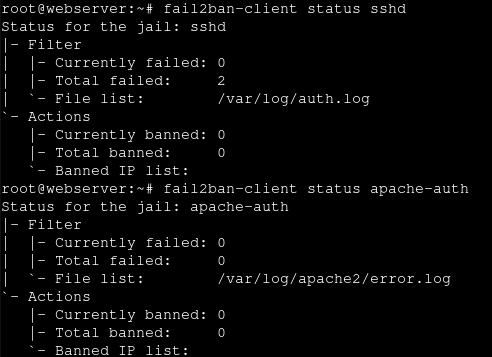
\includegraphics[width=1\textwidth]{fail2banWeb.png}
  \caption[a]{fail2ban jails for services in the Web machine (apache-auth is just one of the several apache jails we enabled).}\label{fig:7}
\end{minipage}%
\begin{minipage}{.5\textwidth}
  \centering
  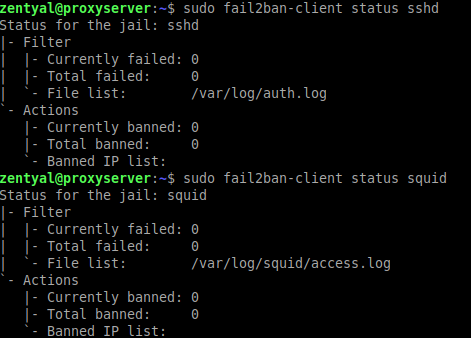
\includegraphics[width=1\textwidth]{fail2banProxy.png}
  \caption[a]{fail2ban jails for services in the Proxy machine.}\label{fig:7}
\end{minipage}%
\end{figure}

Please keep also in mind that we know that at least one more process is running on both machines - the \textbf{rsyslog} process for remote logging at log machine in the Internal servers - but this does not require any authentication mechanism so it is not monitored by the tool.
